%========================================================================================
% Latex-Beamer-Template
% TU Dortmund, Informatik Lehrstuhl VII
%========================================================================================
\documentclass[10pt]{beamer}

\usetheme{tufi}
\usepackage{wasysym}
\usepackage[ngerman]{babel}
\usepackage[utf8]{inputenc}
\usepackage{amsmath,amsfonts,amssymb}
\usepackage{graphicx}
\usepackage[T1]{fontenc}
\usepackage{verbatim}
\usepackage[babel,german=quotes]{csquotes}
\usepackage{array}
\usepackage{multirow}
\usepackage{rotating}
\usepackage{pgfpages}
\usepackage[backend=biber]{biblatex}
\bibliography{Literatur.bib}

\newcommand\tabrotate[1]{\begin{turn}{90}\rlap{#1}\end{turn}}
\newcommand\MyBox[2]{
  \fbox{\lower0.75cm
    \vbox to 1.7cm{\vfil
      \hbox to 1.7cm{\hfil\parbox{1.4cm}{#1\\#2}\hfil}
      \vfil}%
  }%
}

%========================================================================================
% Hier Vortragstitel, Autor und Vortragsdatum eintragen
\pdfinfo
{
  /Title       (Zeit-Effizientes Training von Convolutional Neural Networks)
  /Creator     (TeX)
  /Author      (Jessica Bühler)
}


\title{Masterarbeit -- Zeit-Effizientes Training von Convolutional Neural Networks}
\author{Jessica Bühler}
\date{\today}
%========================================================================================

\begin{document}

\frame{\titlepage}

\AtBeginSection[]
{
  \frame<handout:0>[allowframebreaks]
  {
    \frametitle{Übersicht}
    \tableofcontents[currentsection,hideallsubsections]
  }
}

\AtBeginSubsection[]
{
  \frame<handout:0>[allowframebreaks]
  {
    \frametitle{Übersicht}
    \tableofcontents[sectionstyle=show/hide,subsectionstyle=show/shaded/hide]
  }
}

\newcommand<>{\highlighton}[1]{%
  \alt#2{\structure{#1}}{{#1}}
}

\newcommand{\icon}[1]{\pgfimage[height=1em]{#1}}


%=Inhalt=================================================================================
\section{Einführung}

\begin{frame}{}
\begin{figure}
 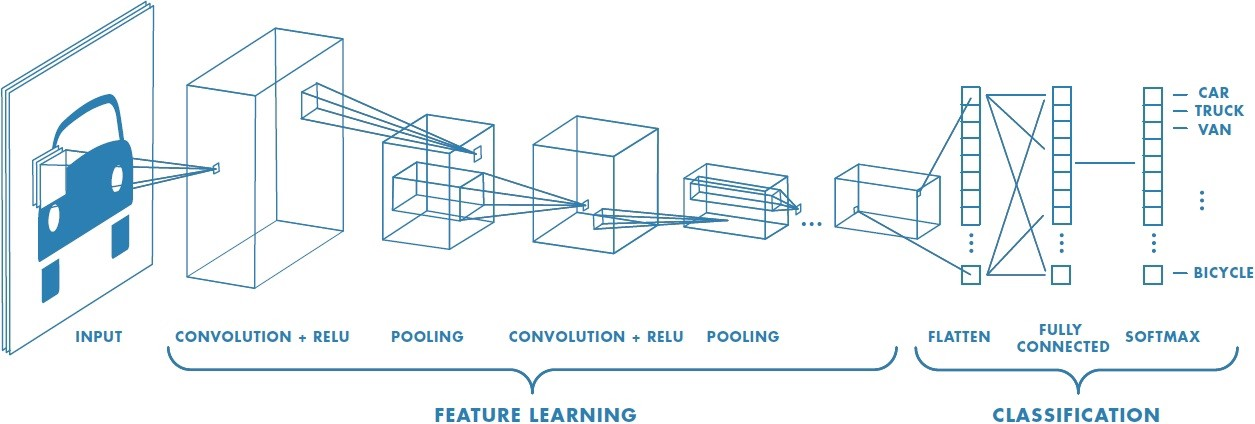
\includegraphics[width=0.8\textwidth]{grafik/cnn.jpeg}
 % cnn.jpeg: 1255x424 px, 72dpi, 44.27x14.96 cm, bb=0 0 1255 424
 \caption{CNN Architecture}
\end{figure}

\end{frame}

\begin{frame}{}
 \begin{figure}
 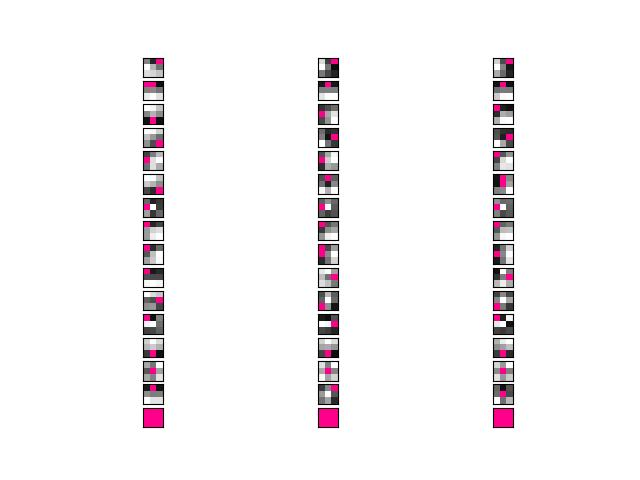
\includegraphics[width=0.9\textwidth]{grafik/module12.jpg}
 % module.conv1.weight_12.png: 640x480 px, 100dpi, 16.26x12.19 cm, bb=0 0 461 346
 \caption{Filtermap}
\end{figure}

\end{frame}

\begin{frame}{}
 \begin{figure}
 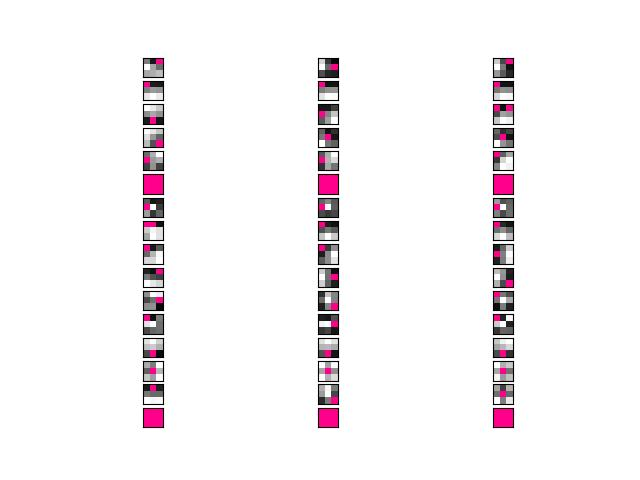
\includegraphics[width=0.9\textwidth]{grafik/module14.jpg}
 % module.conv1.weight_12.png: 640x480 px, 100dpi, 16.26x12.19 cm, bb=0 0 461 346
 \caption{Filtermap}
\end{figure}

\end{frame}

\begin{frame}{}
 \begin{figure}
 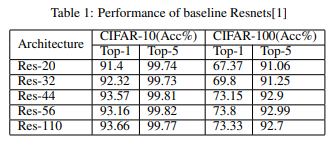
\includegraphics[width=0.8\textwidth]{grafik/resnet.png}
 % resnet.png: 336x148 px, 72dpi, 11.85x5.22 cm, bb=0 0 336 148
 \caption{Resnet Accuracy}
\end{figure}

\end{frame}

\begin{frame}{}
 Forschungsfrage: Lässt sich anhand der Menge an geprunten Daten und eventuell weiterer Daten vorhersagen, wie tief ein Netz sein sollte um eine bestimmte Acuuracy zu erreichen. Schrittweise und möglichst schnell 
\end{frame}

\begin{frame}{}
Ab welcher Tiefe brauchen wir zusätzliche Methoden um das Overfitting unter Kontrolle zu bringen
\end{frame}



\end{document}
